\section{Interface}
A fixity storage must persist any kind of fixity information, in my thesis SHA256 values, for longterm and guarantee that the persisted content is unaltered until retrieval of the content. I have chosen the Ethereum network as a medium for persisting file fixity information, see Section \ref{sec:storage-medium} for my reasoning. In Figure \ref{fig:lifecycle} the lifecycle of fixity information is presented, where at some point in time the information is ingested into the storage and after a certain time interval the information is fetched and compared to the retrieved SHA256 value from the digital object of the archive. If both cryptographic hashes match, the object is guaranteed to be unaltered. 
\begin{figure}[b]
    \label{fig:lifecycle}
    \centering
    \caption{Example of a fixity storage}
    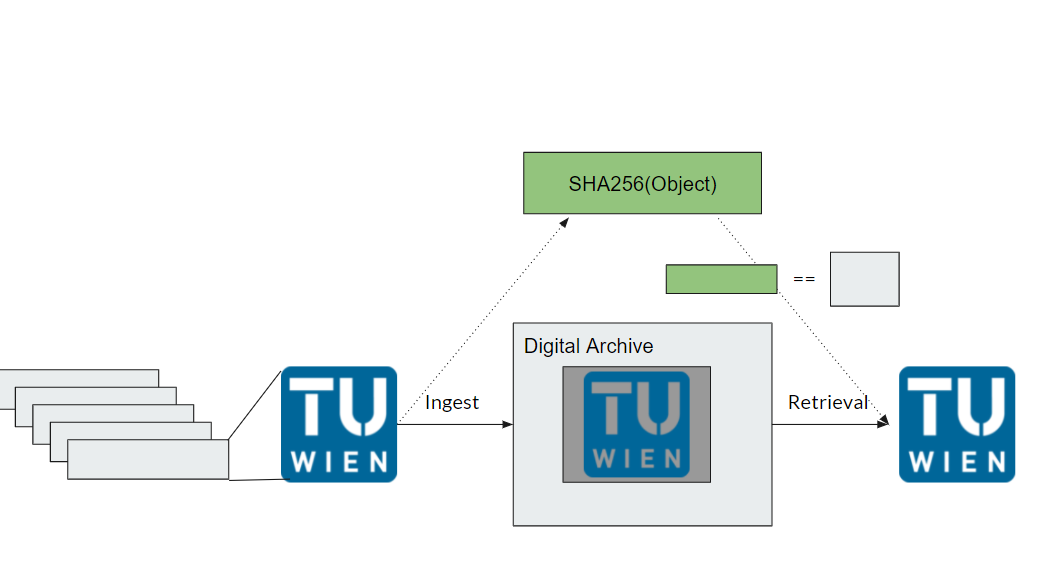
\includegraphics[width=0.75\textwidth]{lifecycle.png}
\end{figure}
\section{Implementation}
The fixity storage presented in this thesis is implemented in Solidity, a programming language designed for the EVM, see Section \ref{sec:evm}.
The basic functionality of the smart contract, as described in Section \ref{sec:approach} can be seen in the source code presented in Listing \ref{lst:fixity-storage}
\begin{lstlisting}[language=Solidity,caption={MVP source code of the fixity storage deployed on the Ropsten test network https://ropsten.etherscan.io/address/0x18648B486Bd6B771DB957590E988A2464F22BfCd TODODODODO},label={lst:fixity-storage}]
    \label{lst:fixity-storage}
// SPDX-License-Identifier: MIT
pragma solidity >=0.4.22 <0.9.0;

contract FixityStorage {
  mapping(uint32=>bytes32) pools;
  address creator;

  constructor()public{
    creator = msg.sender;
  }

  function getPoolHash(uint32 poolId) public view returns(bytes32) {
      return pools[poolId];
  }

  function setPoolHash(uint32 poolId, bytes32 poolHash) public {
    require(msg.sender==creator);
    pools[poolId]=poolHash;
  }
}
\end{lstlisting}
where \textit{getPoolHash(uint32 poolId)} implements a read function; \textit{setPoolHash(uint32 poolId,bytes32 poolHash)} implements create and update function. The mapping type is native in solidity which implements a hash map consisting of a key and a value, where in this case the key is an integer representing the \textit{poolId} and the value is a \textit{bytes32} object representing the SHA256 root hash of the pool. The \textit{poolId} is the reference to the local pool in the digital archive, with which fxiity information can be retrieved for a certain pool from the contract. The solidity language presents a convenient  method to prevent unauthorized calls to the setPoolHash() method, which is \textit{require(msg.sender==creator)}. The native method require is a "guard" function which improves the readability of the smart contract code which fires a REVERT instruction if the condition is not met. The condition in this case is, that only the creator, which is set in the constructor, of the fixity storage is able to creat and alter the information stored on the blockchain.
\section{Deployment}
I utilized trufflesuite\footnote{\url{https://trufflesuite.com/index.html}} to run my deployment of the smart contract. I decided to use truffle to develop, test and deploy the smart contract for the fixity-storage. Truffle is a development environment, testing framework and asset pipeline for blockchains using the Ethereum Virtual Machine. Truffle brings built-in smart contract compilation, linking, deployment and binary management with automated contract testing. The reasoning behind my decision is that, truffle has all the tools needed to implement a smart contract in one package and therefore reduced complexity in the development process. In the first steps I used the user-interface Ganache\footnote{\url{https://trufflesuite.com/ganache/index.html}} to get a better feeling for the ethereum blockchain, see Figure \ref{fig:ganache}.
\begin{figure}[h]
    \label{fig:ganache}
    \caption{Ganache, an interactive user interface for the ethereum blockchain.}
    \centering
    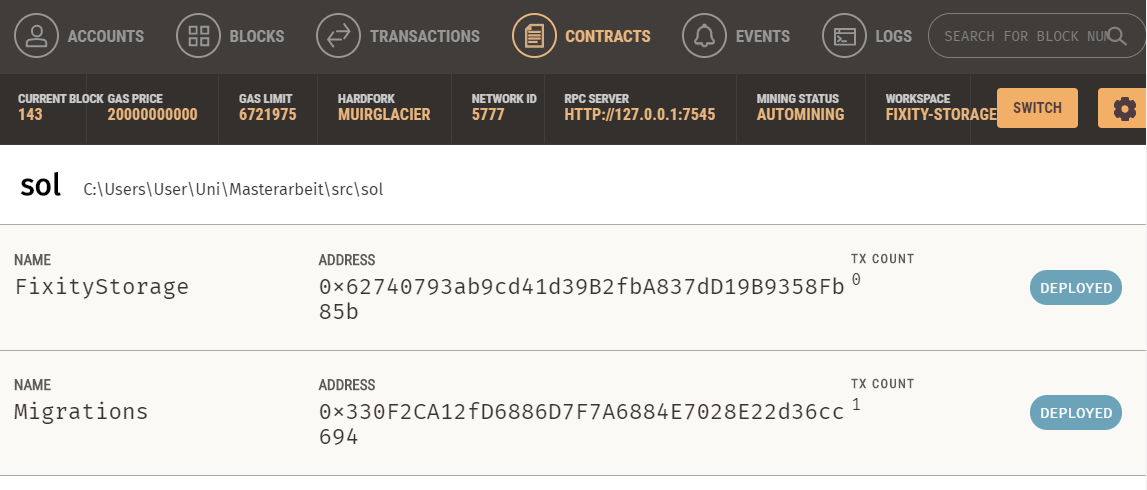
\includegraphics[width=0.7\textwidth]{ganache.png}
\end{figure}
It allows you to click through your smart contract and look at the state variables or functions to validate that your smart contract was successfully deployed. Ganache has a massive disadvantage when doing high throughput computing, it seems that it is no suited to perform 10000 transactions in a python for loop. Therefore I only used it in the beginning of the experiment where I only persisted about 10 objects at a time without problems. For high throughput computing, truffle offers a command line tool to interact with the blockchain. The command line tool was resistent and showed no weakness when persisting 10000 objects.
Truffle also allows to config other networks, e.g. the ropsten test network, which can be defined as a parameter in the deployment process. The deployment requires to have some ether token in your account to pay the miner to integrate your smart contract in a block. 
Truffle offers some utility regarding automated deployment, which are migrations. Migrations are JavaScript files, which are responsible for staging the deployment tasks and running deployment scripts. I used the migrations feature in order to interact with various Ethereum networks, in my case the Ropsten test network and a local test environment. The migrations feature requires to have an smart contract deployed on the blockchain, which causes additional cost (191943 gas) to the fixity storage. 
The deployment cost of the smart contract can be calculated as follows:
\begin{equation}\label{eq:gas-cost}
    C = G_{transaction} + G_{txcreate} + Contract_{bytesize}*G_{codedeposit} + G_{txdatanonzero} * Tx_{bytesize}
\end{equation}
where \textit{$G_{transaction}$} is the base cost for a transaction; \textit{$G_{txcreate}$} is the operation used to create a smart contract; \textit{$G_{codedeposit}$} is the gas cost for each byte of the compiled bytecode of the smart contract; \textit{$G_{txdatanonzero}$} is 16 gas foreach byte in the compiled bytecode of a transaction; \textit{$Contract_{bytesize}$} is the size of the compiled bytecode of the contract; and \textit{$Tx_{bytesize}$} is the size of the compiled bytecode of the transaction, see Section \ref{sec:costs} for the exact gas amount foreach transaction.
The amount of gas consumed by the deployment of the decentralized fixity storage is 164779 gas.
The location of the fixity storage on the blockchain is \textit{0x18648B486Bd6B771DB957590E988A2464F22BfCd TODODODO}, where additional infos or the code can be read.
\section{Authorized Access}
In solidity one can require a certrain address to acess a function, the keyword requires can be used  so that a transaction from a unknown address can be reverted and only the owner of the creator address can update the mapped SHA256 values in the smart contract. An interestng topic is also how the private key in the archive may be managed, which is not part of this thesis but something like a multisignature wallet may be used to split the responsibility of the owner address in the contract. Since the entity which controls the private key of the smart contract is able to perform update operations which can lead to unwanted actions. In the worst case, an unwanted action may be ignored, since the older value is not deleted on the blockchain. Therefore the key usermanagement of the smart contract can be used as a next steps in further research. For this thesis I assume that the private key is well managed and each transaction coming from the master address is legit.